\documentclass[border=10pt,tikz]{standalone}
\usepackage{tikz}
\usetikzlibrary{positioning,arrows.meta}
\begin{document}
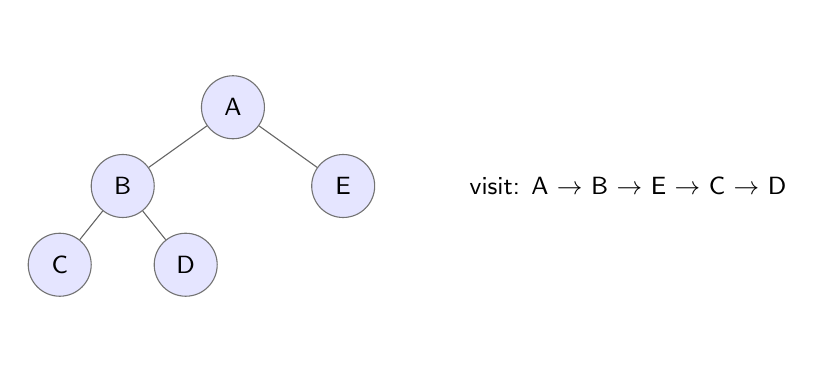
\begin{tikzpicture}[
  font=\sffamily\small,
  every node/.style={circle, draw=black!55, line width=0.4pt, minimum size=8mm, fill=blue!10, inner sep=0pt},
  edge/.style={draw=black!60, line width=0.4pt}
]
\node (a) at (0, 2)    {A};
\node (b) at (-1.4, 1) {B};
\node (e) at (1.4, 1)  {E};
\node (c) at (-2.2, 0) {C};
\node (d) at (-0.6, 0) {D};

\draw[edge] (a) -- (b);
\draw[edge] (a) -- (e);
\draw[edge] (b) -- (c);
\draw[edge] (b) -- (d);

\node[draw=none, fill=none, anchor=west] at (3, 1) {visit: A $\to$ B $\to$ E $\to$ C $\to$ D};
\end{tikzpicture}
\end{document}
